\section{Evaluations on case studies\label{section:evaluation-experiments-on-case-studies}}

QSM and ASM were evaluated on three different case studies of varying complexity. The first one is a mine pump system inspired from~\cite{Joseph:1996} and often used as a ``benchmark'' in the literature. The second case study refers to an extended version of the train system used here as a running example. The third one is a phone system handling communications between a caller and a callee.

Section \ref{subsection:evaluation-case-study-methodology} details the evaluation methodology. Section \ref{subsection:evaluation-isis-modeling-session} illustrates a typical modeling session in the ISIS tool on the mine pump system. The subsequent sections then further discuss the impact observed on model adequacy, number of scenario questions and induction time of the different induction features, such as using an oracle or the Blue-fringe heuristics.

\subsection{Evaluation methodology\label{subsection:evaluation-case-study-methodology}}

Beyond a practical evaluation of our tool-supported approach to multi-view LTS synthesis, our objective was to assess the impact of constraining induction through fluents, models of external components, domain descriptions and goals. Such impact was measured in terms of the number of generated scenario questions and the adequacy of the synthesized models. Induction time was also measured so as to check that fast interactions with the oracle are observed.

For each case study, we proceeded in two steps:
\begin{enumerate}
\item\label{stepA}
\begin{enumerate}
\item\label{CondA} Design a scenario collection allowing for meaningful subsequent comparison, that is, sufficiently rich to allow an adequate system LTS to be induced under one setting of the experiment at least (see hereafter).
\item\label{CondB} Define a common set of fluent definitions identifiable from this scenario collection. From this set of fluents, define a common set of domain properties and goals.
\end{enumerate}
\item\label{stepB} Evaluate the techniques on this scenario collection, without and then with fluents, goals, domain descriptions, or models of external components.
\end{enumerate}

In Step~\ref{stepA}, the richness condition on the scenario collection~(a) amounts to require the collection to be structurally complete; every transition in the target system LTS must occur in at least one scenario (see Section \ref{section:inductive-background}). The ISIS tool was used to incrementally set up such a scenario collection (see Section \ref{section:tool-support-isis}):
\begin{itemize}
\item An initial set of scenarios that end-users would typically provide was first selected.
\item By generating scenario questions, adding domain properties and goals, and validating the induced LTS, additional scenarios were found that were initially missing. 
\item Some of these scenarios were added to the collection for the comparisons in Step~\ref{stepB}. Added scenarios have been selected so as to reach a structurally complete collection of scenarios without making it too rich.
\end{itemize}

\begin{table}[H]
\centering
\begin{tabular}{|l||c|c|c||c|c|c|}\hline
Problem  & Events & States & Trans. & $|S^+|$ & $|S^-|$ & Avg. length\\\hline\hline
Mine Pump& 8      & 10     & 13          & 3     & 0     & 8\\\hline
Train    & 13     & 17     & 23          & 3     & 0     & 9\\\hline
Phone    & 16     & 23     & 33          & 6     & 4     & 11\\\hline
\end{tabular}
\caption{Sizes of the case studies.\label{CaseStudies}}
\end{table}

The size of the scenario collection resulting from Step~\ref{stepA} is shown in Table~\ref{CaseStudies}. $|S^+|$ and $|S^-|$ denote the number of positive and negative scenarios, respectively. The average scenario length is reported in the last column. The size of the target system LTS are also reported in terms of number of different event labels (alphabet size), states, and transitions. 

In order to measure the number of generated scenario questions in Step \ref{stepB}, an oracle was implemented to simulate the end-user. This oracle knows the system LTS for each problem and correctly classifies generated scenario as positive or negative. Note that this is a strong assumption on the oracle, especially when played by an end-user in practice; this issue has been discussed in Section~\ref{section:inductive-discussion}.

The next section illustrates how the ISIS tool were used to build the scenarios, domain properties and goals for the Mine Pump system. Then, results of evaluation experiments will be detailed.

\subsection{Modeling the Mine Pump system with ISIS\label{subsection:evaluation-isis-modeling-session}}

This section shows the ISIS tool in action on a classical Software Engineering benchmark. We consider the following simplified problem statement for the Mine Pump exemplar \cite{Joseph:1996}:
\begin{quotation}
\emph{Water percolating into a mine is collected in a sump to be pumped out of the mine. The water level sensor detects when water is above and below a specific level. A pump controller switches the pump on when the water goes above this level and off when it goes below this level. To avoid the risk of explosion, the pump must be operated only when the methane level is below some critical level.}
\end{quotation}

The tool allows specifying positive and negative scenarios. In addition, if available, other kinds of knowledge can be captured. Such information includes fluents, state machines of legacy components or safety properties to be met by the system.

Fig.~\ref{image:minepump-initial-scenarios} shows two positive scenarios initially drawn from the description above. As stated in Chapter~\ref{chapter:inductive-synthesis}, our inductive technique make the built-in assumption that such input scenarios start in the same initial state. The submitted scenarios thus implicitly specify that the water level is low and the methane level is below the critical level. 

\begin{figure}
\centering
\scalebox{0.75}{
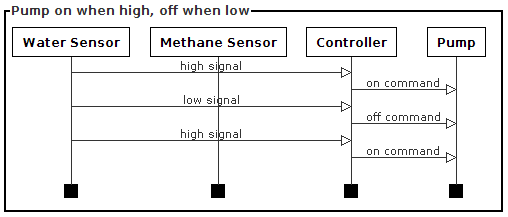
\includegraphics[trim=0mm 0mm 0mm 0mm, clip]{src/5-evaluation/casestudy/PumpOnWhenHighAndOffWhenLow}
}
\scalebox{0.75}{
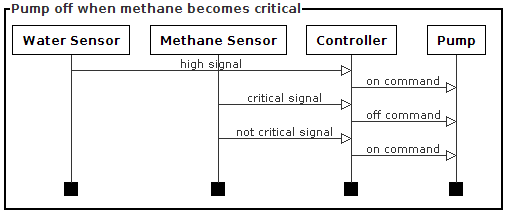
\includegraphics[trim=0mm 0mm 0mm -5mm, clip]{src/5-evaluation/casestudy/PumpOffWhenCriticalMethane}
}
\caption{Initial scenarios for the Mine Pump system\label{image:minepump-initial-scenarios}.}
\end{figure}

The first positive scenario illustrates that the pump should be turned on by the controller when the water level is high and turned off when the water level is low. If the water gets high once again, the controller simply turns the pump on in response. 

The second scenario shows that the pump should be turned off when the methane level becomes critical. As the water is high, the pump is switched back on when the methane level becomes non critical.

\subsubsection*{Running QSM with these two scenarios}

QSM is ran a first time with these two scenarios as input. For our case-study evaluations, QSM was actually used with the Blue-Fringe heuristic and a consolidation threshold of 1 (see Section~\ref{BlueFringe}). This means that two states of the PTA are considered for merging only if they share at least one outgoing event. Such consolidation threshold drastically reduces the number of possible scenario questions; generated questions also tend to be guided by more evidence, which fits the intuition. In our experience, doing so results in a conservative state merging approach that is well suited for building a new specification from scratch.

With such a configuration, only one scenario question is submitted for classification. It is illustrated in Fig.~\ref{image:minepump-scenario-question} and can be rephrased as: ``\emph{after having switched the pump off because of a critical level of methane, may the controller switch the pump on if the water becomes high once again?}''. At least two reasons support the rejection of such a scenario:

\begin{figure}
\centering
\scalebox{0.75}{
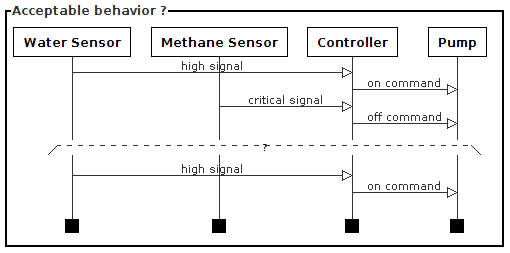
\includegraphics[trim=0mm 0mm 0mm 0mm, clip]{src/5-evaluation/casestudy/MayWaterBeHighTwice}
}
\caption{A first scenario question submitted by QSM on the Mine Pump case study.\label{image:minepump-scenario-question}}
\end{figure}

\begin{itemize}
\item A domain property prevents the water from becoming high twice in a row. Observing two ``high'' signals from the water sensor consecutively brings our attention to the fact that the scenario should probably be rejected.

This domain property might be formally captured in two ways: either by a legacy LTS for the water sensor (see Fig.~\ref{image:minepump-water-sensor-lts}) or by a declarative domain property.
\begin{figure}[H]
\centering
\scalebox{0.4}{
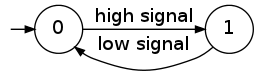
\includegraphics[trim=0mm 0mm 0mm 0mm, clip]{src/5-evaluation/casestudy/WaterSensorLTS}
}
\label{image:minepump-water-sensor-lts}
\end{figure}

If the declarative option is chosen, the following LTL safety property can be used to capture the fact that the ``high water'' signal is only observed provided that the current water level is low:
\begin{align*}
&\mbox{DomProp[Water]} = \circ(\mbox{high signal}) \Rightarrow \neg \mbox{HighWater}\\
&\mbox{fluent HighWater} = \textless \{\mbox{high signal}\}, \{\mbox{low signal}\} \textgreater \mbox{initially \emph{false}}
\end{align*}

\item In addition, the level of methane is still critical in the second part of the scenario question. In such a situation the controller may not switch the pump on.

This second rejection reason might be captured through the following safety goal.
\begin{align*}
&\mbox{Avoid[PumpOnWhenMethane]} = \mbox{CriticalMethane} \Rightarrow \circ(\neg \mbox{PumpOn}) \\
&\mbox{fluent CriticalMethane} = \textless \{\mbox{critical signal}\}, \\ 
&\{\mbox{not critical signal}\} \textgreater\mbox{initially \emph{false}} \\
&\mbox{fluent PumpOn} = \textless \{\mbox{on command}\}, \{\mbox{off command}\} \textgreater \mbox{initially \emph{false}}
\end{align*}

\end{itemize}

Note that the scenario may simply be rejected without further explanation. As illustrated above, the rejection of a scenario is a rich opportunity to declare state variables and identify requirements and domain properties. However such more formal steps are optional and may simply be bypassed by non-experts. Not specifying fluents, domain properties and goals typically lead to more scenario questions.

In our modeling session, only the \artifact{CriticalMethane}, \artifact{HighWater} fluents above were defined. No further scenario questions were submitted for classification. The resulting LTS for the pump controller agent is illustrated in Fig.~\ref{image:minepump-controller-1-annotated}.

\begin{figure}
\centering
\scalebox{0.3}{
  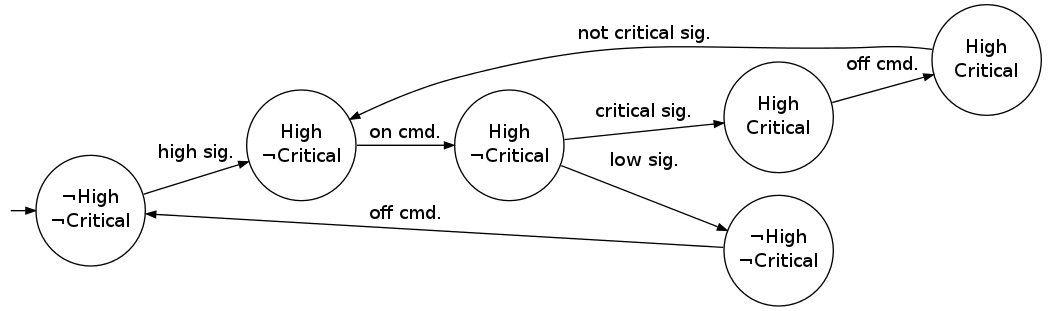
\includegraphics[trim=0mm 0mm 0mm 0mm, clip]{src/5-evaluation/casestudy/controller-1-annotated}
}
\caption[The annotated LTS of the Pump Controller]{The annotated LTS of the Pump Controller\label{image:minepump-controller-1-annotated}. Here ``sig.'' stands for ``signal'' and ``cmd.'' stands for ``command'', ``High'' stands for ``HighWater'' and ``Critical'' for ``Critical Methane''.}
\end{figure}

\subsubsection*{A second modeling step}

At this step various choices can be made:
\begin{itemize}
\item More positive and negative scenarios can be added to the initial scenario collection. QSM is then ran once again and generates new scenario questions.
\item The consolidation threshold of Blue-fringe can be lowered. This results in a more aggressive state merging approach, leading to new scenarios to classify as positive or negative system behaviors. Doing so triggers for further identification of domain properties and goals.
\item Synthesized state machines may be decorated with fluent invariants and inspected by experts. New positive scenarios are typically added to the scenario collection so as to cover missing behaviors. New negative scenarios can be added when over-generalization is detected.
\item Additional synthesis and/or analysis tools can be launched on the specification, such as an animator or a model checker. In particular, the ISIS tool supports the inference of goals from scenarios~\cite{Damas:2006, Damas:2011}.
\end{itemize}

The last option was chosen in our case, the ISIS tool being requested to infer maintain goals from the annotated scenarios. Only one property was inferred and submitted for classification:
\begin{align*}
\square(\mbox{HighWater} \vee \neg \mbox{CriticalMethane})
\end{align*}

This property states that either the water is high or the methane is below the critical level. It has to be rejected as those two phenomena are independent of each other. A counterexample scenario must illustrate a situation where the water level is low while the level methane is critical:
\begin{align*}
\square(\neg \mbox{HighWater} \wedge \mbox{CriticalMethane})
\end{align*}

Fig.~\ref{image:minepump-scenario-3} provides such counterexample where the ``critical signal'' event is observed in the initial state. The pump may then be switched on only if the methane level is below the critical level.

\begin{figure}
\centering
\scalebox{0.75}{
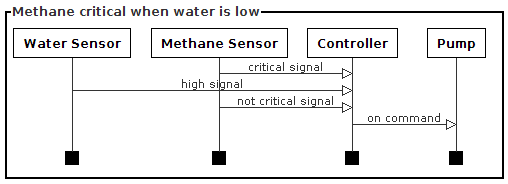
\includegraphics[trim=0mm 0mm 0mm 0mm, clip]{src/5-evaluation/casestudy/MethaneCriticalWhenWaterIsLow}
}
\caption{The methane level may become high when the water is low.\label{image:minepump-scenario-3}}
\end{figure}

\subsubsection*{Running QSM a second time}

As a new scenario is available, QSM is ran so as to obtain revised agent state machines. With a consolidation threshold of 1, no scenario question is submitted for classification. The revised LTS state machine of the pump controller is shown in Fig.~\ref{image:minepump-controller-2-annotated}.
\begin{figure}
\centering
\scalebox{0.27}{
  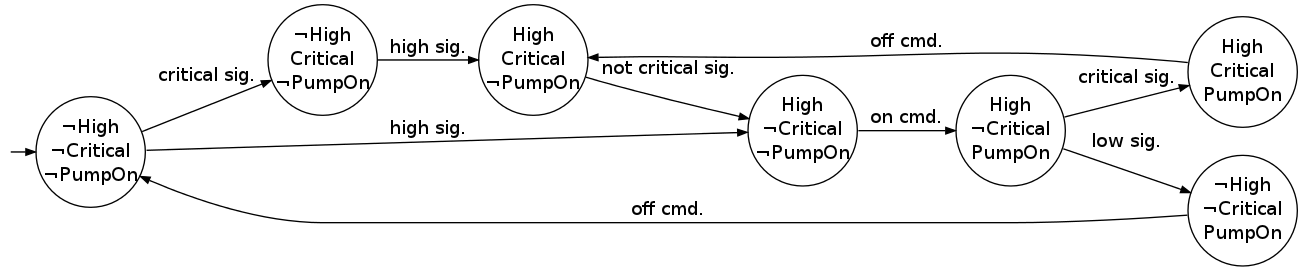
\includegraphics[trim=0mm 0mm 0mm 0mm, clip]{src/5-evaluation/casestudy/controller-2-annotated}
}
\caption{A second version of the Pump Controller LTS\label{image:minepump-controller-2-annotated}}
\end{figure}

A manual inspection of this state machine showed that only one transition was missing, that would allow the methane to become critical then not critical from the initial state. This was fixed by simply adding such a loop at the beginning of the third scenario and running QSM once again (see Fig.~\ref{image:minepump-scenario-3-bis}).

\begin{figure}[H]
\centering
\scalebox{0.75}{
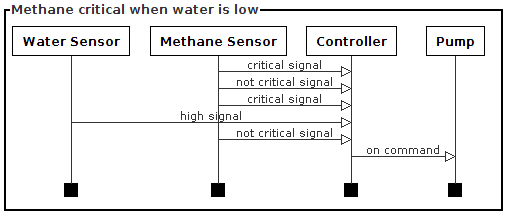
\includegraphics[trim=0mm 0mm 0mm 0mm, clip]{src/5-evaluation/casestudy/MethaneCriticalWhenWaterIsLow2}
}
\caption{Third scenario revised to include a loop through the methane events.\label{image:minepump-scenario-3-bis}}
\end{figure}

\subsubsection*{Inferring goals}

From fluent definitions and the four available scenarios (3 positive and 1 negative), the tool was requested to infer goals. Three of them were kept as typical requirements of the mine pump system:
\begin{itemize}

\item Maintain[PumpOn When HighWater and Not Critical Methane]
\begin{align*}
&\mbox{HighWater} \wedge \neg \mbox{CriticalMethane} \Rightarrow \circ(\mbox{PumpOn})
\end{align*}

\item Avoid[PumpOn When LowWater]
\begin{align*}
&\neg \mbox{HighWater} \Rightarrow \circ(\neg \mbox{PumpOn})
\end{align*}

\item Avoid[PumpOn When CriticalMethane]
\begin{align*}
&\mbox{CriticalMethane} \Rightarrow \circ(\neg \mbox{PumpOn})
\end{align*}

\end{itemize}

These goals were used to prune the induction in controlled experiments. The resulting specification was considered rich enough; it enabled a deeper evaluation of our inductive algorithm by controlling various parameters such as the number of injected goals. A similar process were used on the two other case studies. The results are described in the next sections.

%%%%%

\subsection{RPNI search order vs. Blue-fringe strategy\label{subsection:evaluation-bluefringe-on-casestudies}}

Table~\ref{RPNI:Blue-fringe} reports the results obtained when running QSM with the RPNI search order and the Blue-fringe heuristics, respectively. In the sequel, these two settings will be denoted by QSM-rpni and QSM-fringe, respectively. The comparisons are made without additional knowledge to constrain induction. 

\begin{table}[H]
\centering
\begin{tabular}{|l||l||c|c|c|}\hline
Problem   & Algorithm   &$Q^+$&$Q^-$& Model adequacy\\\hline\hline
Mine Pump & QSM-rpni    & 1   & 30  & missing/unallowed traces\\\cline{2-5}
          & QSM-fringe  & 1   & 4   & adequate model\\\hline
Train     & QSM-rpni    & 4   & 83  & adequate model\\\cline{2-5}
          & QSM-fringe  & 5   & 5   & adequate model\\\hline
Phone     & QSM-rpni    & 5   & 171 & missing/unallowed traces\\\cline{2-5}
          & QSM-fringe  & 5   & 19  & missing/unallowed traces\\\hline
\end{tabular}
\caption{RPNI search order versus Blue-Fringe strategy for QSM.\label{RPNI:Blue-fringe}}
\end{table}

The table shows the number of queries the oracle had to answer together with a binary measure of model adequacy. $Q^+$ and $Q^-$ denote the number of accepted and rejected scenario questions, respectively. The model is said to be \emph{adequate} if it matches the known target LTS, formally if the two models are trace equivalent (see Definition \ref{definition:trace-equivalence}). 

The following main observations can be made from these results:
\begin{itemize}
\item The large number of generated questions makes QSM-rpni unusable with end-users on bigger systems. In contrast, the number of rejected scenario questions is drastically reduced thanks to the Blue-fringe search strategy. 
\item In the phone system, an adequate system LTS cannot be synthesized with the sole use of the initial scenario collection and scenario questions. Wrong generalizations do occur; some states are merged whereas they need to be distinguished. A richer scenario collection would allow to correctly identify the target model; remember, however, that the initial collections have been chosen so as to observe the gain in adequacy when injecting fluent definitions and goals in the synthesis process.
\item Finally, the number of rejected scenarios tends to be much larger than the number of accepted ones. This observation confirms the usefulness of scenario questions. Negative answers force the induction algorithm to be restarted when an incorrect search path has been taken (see Algorithm~\ref{QSM} in Section~\ref{section:lts-induction-from-mscs}).
\end{itemize}

As the Blue-fringe heuristics appeared by far superior to the RPNI search order, subsequent comparisons were made only with QSM-fringe.

%%%%%

\subsection{Impact of fluent propagation}

In this second evaluation, the synthesis is performed for each case study on an increasing number of fluents among those available.

\begin{table}[H]
\centering
\begin{tabular}{|l||c||c|c|c|}\hline
Problem&Nb. fluents&$Q^+$&$Q^-$&Model adequacy\\\hline\hline
Mine Pump&0&1&4&adequate model\\\cline{2-5}
&1&1&1&adequate model\\\cline{2-5}
&2&1&0&adequate model\\\cline{2-5}
&3&1&0&adequate model\\\hline\hline
Train&0&5&5&adequate model\\\cline{2-5}
&1&5&3&adequate model\\\cline{2-5}
&2&5&3&adequate model\\\cline{2-5}
&3&5&3&adequate model\\\cline{2-5}
&4&5&2&adequate model\\\cline{2-5}
&5&5&0&adequate model\\\hline\hline
Phone&0&5&19&missing/unallowed traces\\\cline{2-5}
&1&5&13&missing/unallowed traces\\\cline{2-5}
&2&6&9&adequate model\\\cline{2-5}
&3&6&4&adequate model\\\hline
\end{tabular}
\caption{Impact of fluent propagation.\label{Fluents:res}}
\end{table}

Table~\ref{Fluents:res} summarizes the influence of fluent decorations to constrain the induction process. The following observations can be made:
\begin{itemize}
\item The number of rejected scenario questions is decreasing as the number of fluents is increasing. Such questions can even disappear when the set of fluent definitions is large enough. 
\item In contrast, for the same induced LTS, the number of accepted scenarios remains the same. Fluent-based state information can only increase the number of incompatible states and hence, reduce the number of rejected scenarios.
\item As seen in the phone system, fluent definitions yield a better model adequacy. Together with the initial scenario collection and the answers to scenario questions, two fluents were sufficient for a trace equivalent model to be found.
\end{itemize}

%%%%%

\subsection{Impact of goals and domain properties}

From a scenario collection and fluent definitions, the ISIS tool can automatically infer a variety of requirements and domain properties using an inference technique described in \cite{Damas:2006, Damas:2011} (see Section~\ref{section:tool-support-isis}). This feature was used to measure the impact of goals and domain properties on the induction process.

For the Mine Pump system, three important requirements were inferred automatically, e.g.,
\begin{quote}
\emph{When the water level is below the low water threshold, the pump controller must immediately set the pump to ``off''.}
\end{quote}

For the Big Train system, three requirements and two domain properties were inferred automatically, e.g.,
\begin{quote}
\emph{The train may never run at high speed when it comes near a station.}
\end{quote}

For the Phone system, three requirements were inferred automatically, e.g.,

\begin{quote}
\emph{When the caller hangs up, the connection should immediately be closed.}
\end{quote}

Those inferred properties were used in turn to incrementally constrain the induction process. Table \ref{Properties:res} shows the results obtained.

\begin{table}
\centering
\begin{tabular}{|l||c||c|c|c|}\hline
Problem   & Nb. properties &$Q^+$&$Q^-$& Model adequacy\\\hline\hline
Mine Pump & 0              & 1   & 4   & adequate model\\\cline{2-5}
          & 1              & 1   & 0   & adequate model\\\cline{2-5}
          & 2              & 1   & 0   & adequate model\\\cline{2-5}
          & 3              & 1   & 0   & adequate model\\\hline\hline
Train     & 0              & 5   & 5   & adequate model\\\cline{2-5}
          & 1              & 5   & 3   & adequate model\\\cline{2-5}
          & 2              & 5   & 3   & adequate model\\\cline{2-5}
          & 3              & 5   & 3   & adequate model\\\cline{2-5}
          & 4              & 5   & 2   & adequate model\\\cline{2-5}
          & 5              & 5   & 0   & adequate model\\\hline\hline
Phone     & 0              & 5   & 19  & missing/unallowed paths\\\cline{2-5}
          & 1              & 6   & 6   & adequate model\\\cline{2-5}
          & 2              & 6   & 4   & adequate model\\\cline{2-5}
          & 3              & 6   & 4   & adequate model\\\hline
\end{tabular}
\caption{Impact of inferred properties on induction.\label{Properties:res}}
\end{table}

Compared with fluent injection, similar observations can be made, that is, goals help reaching a better model adequacy while reducing the number of rejected scenario questions. Goals and domain properties are however seen to be slightly more powerful than fluents. With one single goal, there are no rejected scenario questions anymore in the Mine Pump system; the LTS generated for the Phone system is now adequate.

%%%%%

\subsection{Combined use of fluents, properties and external components}

Table~\ref{All:res} shows the results of QSM-fringe induction constrained with all fluents, goals and domain properties, and foreign component(s) available in each case study. (The fact that the number of fluents and goals is the same for each case study is purely coincidental.)

For each problem, the first line corresponds to the simplest approach, that is, QSM with the RPNI search order and no domain knowledge. The second line shows how much is gained when the various techniques are combined to constrain the interactive synthesis process. For example, QSM-fringe inferred an adequate model for the phone system with only 3 rejected scenario questions; in contrast, 172 rejected questions were not sufficient to find such model with QSM-rpni.

\begin{table}[H]
\centering
\begin{small}
\begin{tabular}{|l||c|c|c|c||c|c|c|}\hline
Problem   & Search      & Fl. & Goals & Comp. &$Q^+$&$Q^-$& Adequacy\\\hline\hline
Mine Pump & QSM-rpni    & 0   & 0     & 0     & 1   & 30  & not adequate\\\cline{2-8}
          & QSM-fringe  & 3   & 3     & 2     & 1   & 0   & adequate\\\hline\hline
Train     & QSM-rpni    & 0   & 0     & 0     & 4   & 83  & adequate\\\cline{2-8}
          & QSM-fringe  & 5   & 5     & 2     & 5   & 0   & adequate\\\hline\hline
Phone     & QSM-rpni    & 0   & 0     & 0     & 5   & 172 & not adequate\\\cline{2-8}
          & QSM-fringe  & 3   & 3     & 1     & 7   & 3   & adequate\\\hline
\end{tabular}
\end{small}
\caption{Combining fluents, properties and external components to constrain induction\label{All:res}.}
\end{table}

%%%%%

\subsection{Impact of using additional control information\label{subsection:evaluation-casestudies-asm}}

To measure the impact of using a hMSC as input of the synthesis process, ASM has been evaluated on an extended version of our train system. The evaluation protocol is slightly different from the one presented in the previous section.
\begin{itemize}
\item The target model of the train system was first been built using ISIS, yielding a system LTS of 19 states and 10 events (see Figure~\ref{image:case-studies-big-train-2}). 
\item A typical collection of scenarios was also built for the system and represented as an augmented PTA, yielding 9 positive and 5 negative scenarios for a total of 55 states.
\item Using the target LTS, a few state pairs of the PTA were identified as corresponding to the same system state, and immediately merged. This early state merging occurs before launching the inductive algorithm. The automaton resulting from this phase was then given as input to ASM; its performance was then evaluated (see below). The algorithm generalizes the automaton by merging additional state pairs under the control of the negative scenarios.
\end{itemize}

\begin{figure}
\centering
\scalebox{.38}{\includegraphics*{src/5-evaluation/images/case-studies-big-train-2}}
\caption{Target model of the train system.\label{image:case-studies-big-train-2}}
\end{figure}

The early state merging phase simulates the control information typically offered by a hMSC. State pairs of the PTA that are merged early have been chosen following a ``loop identification'' heuristic, representative of the way such a specification is incrementally built by an end-user using an hMSC. 

For instance, opening and then closing the doors from the initial state naturally returns to the initial state (see the loop between states 0 and 2 in Figure~\ref{image:case-studies-big-train-2}). Some loops are less obvious to identify from the scenarios, e.g., the sequence of events ($leaving$, $high$, $approaching$, $low$, $at station$) forms a loop starting from state 3. 

Equivalent state pairs identified this way were classified in four categories, according to the expected difficulty for an end-user to discover them in the scenarios. ASM was then evaluated on increasing proportions of such state pairs being merged early: 3\%, 6\%, 10\% and 15\%. This simulates the use of an increasingly rich hMSC as input to the induction process. 

\begin{table}[H]
\centering
\small
\begin{tabular}{|l|c|c|}\hline
Algorithm& \% equivalent state pairs merged early &Accuracy\\\hline\hline
RPNI      & -    & 0.55\\\hline
Blue-fringe& -   & 0.83\\\hline
ASM       & 0 \%  & 0.55\\\cline{2-3}
          & 3 \%  & 0.71\\\cline{2-3}
          & 6 \%  & 0.73\\\cline{2-3}
          & 10 \% & 0.88\\\cline{2-3}
          & 15 \% & 0.90\\\hline
\end{tabular}
\caption{Classification accuracy obtained with different setups on the train case study.\label{RE:experesults}}
\end{table} 

Table~\ref{RE:experesults} compares the accuracy of the LTS learned using RPNI, Blue-fringe and ASM, with an increasing percentage of equivalent PTA state pairs merged early. (Remember that in our current implementation, ASM uses the same search order as RPNI and does not benefit from the Blue-fringe heuristic -- see Section \ref{section:inductive-from-hMSC}).

As seen in Table~\ref{RE:experesults}, the reported model adequacy is no longer a binary measure here. Instead, an accuracy measure of the learned model is reported as the average classification rate computed over 10 independent test samples. Each of these samples contains 80 positive or negative scenarios randomly drawn from the target LTS. The classification rate corresponds to the percentage of these scenarios correctly classified by the learned model. 

This experiment shows that enriching the input given to ASM leads to better accuracy, which is expected. Interestingly, ASM outperforms Blue-fringe when such control information gets rich enough. In the experiment, it already occurs when 10\% of the state pairs known to correspond to the same system state are merged ahead of the induction itself.

The results also show that no algorithm was able to perfectly identify the target model on such sparse samples. In order to isolate the effect of injecting control information in the induction process, only a few negative scenarios were used as source of negative information while other sources do exist, such as fluents and goals.

%%%%%

\subsection{Induction time}

Only the adequacy and the number of generated scenario questions have been discussed so far. The induction time was also systematically monitored in our evaluations as it drives the usability of QSM in practice. 

All experiments reported in this section were conducted on a Pentium IV, 1.8 GHz, 512Mb with Java 5.0. When using QSM, our tests showed that the maximum time between two scenario questions was 40ms for the bigger case study. The interactions with the end-user are performed in real-time. No performance problems are expected with respect to user interactivity for typical sizes of requirement models, even if larger than those considered here by an order of magnitude.

